\documentclass[12pt]{article}
\usepackage[hmargin={1in},vmargin={1in,1in},foot={.6in}]{geometry}   
\geometry{letterpaper}              
\usepackage{color,graphicx}
\usepackage{setspace}
\usepackage{amsmath}
\usepackage{amssymb}
\usepackage{varioref}
\usepackage{textcomp}
\usepackage{textcomp}
\usepackage{mflogo}
\usepackage{wasysym}
\usepackage[normalem]{ulem}
\usepackage{hyperref}

\newcommand{\HRule}{\rule{\linewidth}{0.25mm}}

\usepackage{fancyhdr} % This should be set AFTER setting up the page geometry
\pagestyle{plain} % options: empty , plain , fancy
\lhead{}\chead{}\rhead{}
\renewcommand{\headrulewidth}{.5pt}
\lfoot{}\cfoot{\thepage}\rfoot{}
\newcommand{\txtp}{\textipa}
\renewcommand{\rm}{\textrm}
\newcommand{\sem}[1]{\mbox{$[\![$#1$]\!]$}}
\newcommand{\lam}{$\lambda$}
\newcommand{\lan}{$\langle$}
\newcommand{\ran}{$\rangle$}
\newcommand{\type}[1]{\ensuremath{\left \langle #1 \right \rangle }}

\newcommand{\bex}{\begin{exe}}
\newcommand{\eex}{\end{exe}}
\newcommand{\bit}{\begin{itemize}}
\newcommand{\eit}{\end{itemize}}
\newcommand{\ben}{\begin{enumerate}}
\newcommand{\een}{\end{enumerate}}

\newcommand{\gcs}[1]{\textcolor{blue}{[gcs: #1]}}
\definecolor{Green}{RGB}{10,200,100}
\newcommand{\ndg}[1]{\textcolor{Green}{[ndg: #1]}}
\newcommand{\jd}[1]{\textcolor{red}{[jd: #1]}}

\thispagestyle{plain}

\begin{document}

{\flushright

\vspace{25pt}
Gregory Scontras\\
Noah D.~Goodman\\
Department of Psychology\\
Stanford University\\
Stanford, CA 94305\\[20pt]

\noindent June XXX, 2016\\[20pt]}


\noindent Dear Editor,\\

\noindent We would like to thank you and the three reviewers for your helpful comments on our paper, ``Subjectivity predicts adjective ordering preferences.'' As you will recall, you highlighted the following concerns: 

\ben

\item \emph{Reviewer 2 questioned whether endorsements of `together' paraphrases are indicative of collective interpretations.}

The reviewer's concerns about our \emph{together} paraphrases stem from previous experimental work that suggests some flexibility in \emph{together}'s disambiguating potential. However, this work and ours share a crucial difference: all of the previous work that the reviewer mentions investigates post-VP \emph{together}, whereas we are careful to use post-NP \emph{together} precisely to avoid the reviewer's concerns. We expand on this point in our response to Reviewer 2's points 1 and 4 below.

\item \emph{Reviewer 2 raised alternative accounts of the contextual effects on the interpretation of bare sentences.}

\item \emph{Reviewer 2 raised the possibility of `cumulative' construals in the interpretation of bare sentences.}

\item \emph{Reviewer 2 mentioned prior published research that is relevant for Experiment 1.}

We now cite the suggested research and stress that our contribution is indeed a novel one (cf.~our response to Reviewer 2's point 1 below).

\item \emph{Reviewer 2 recommends highlighting the novel contribution of the speaker's epistemic state.}

\item \emph{Reviewer 1 was concerned that the effects of contextual predictability were only tested on a limited set of words and contexts.}

We followed the reviewer's suggestion and ran an additional experiment (\emph{Expt.~4: Generalizing our findings}), which tests the predictions of contextual predictability and speaker knowledge with a much larger set of 25 dimensional adjectives (cf.~our original set of three). The new results replicate our original findings and add nuance to our account, highlighting an additional aspect of the pragmatic calculus of utterance disambiguation: the probability that a specific interpretation would truthfully describe a state of affairs. We expand on this point in our response to Reviewer 1's point 1 below.

\item \emph{Reviewer 1 requested more information about the ratings data to get a better sense of individual response patterns.}

We have replaced most of our bar plots with the more informative violin plots that Reviewer 1 suggested. We expand on this point in our response to Reviewer 1's point 2 below.

\item \emph{Reviewer 3 raised an alternative account of subjects' interpretation of `tall' in regular vs. irregular contexts.}

The reviewer raised the issue of how the likely truth of a given interpretation might affect its probability: interpretations that are more obviously true should be more probable. We explore this idea in our new experiment (\emph{Expt.~4: Generalizing our findings}; cf.~our response to the Editor's point 6 above), and find that an interpretation's probability of being judged true affects that interpretation's overall probability. We expand on this point below in our responses to Reviewer 1's point 1 and Reviewer 3's point 3.

\een


\noindent In the remainder of this letter, we consider in more detail each of the reviewers' concerns.


\newpage

\subsubsection*{Reviewer 1:}

\ben

\item \emph{My largest reservation is that the main result, which is that contextual predictability affects whether an interpretation is distributive or collective, is really only experimentally evaluated (in Experiment 3) for three words (\emph{big}, \emph{heavy}, and \emph{tall}) in one context (moving boxes). The paper would be much stronger if either the number of words were broader, or the contexts were broader.}

We have followed the reviewer's suggestion, investigating contextual predictability and speaker knowledge with a much broader set of predicates (\emph{Expt.~4: Generalizing our findings}). We extended the Cubert paraphrase endorsement paradigm from Expt.~3, testing a total of 25 dimensional adjectives (cf.~the three predicates tested in Expt.~3). We grouped these adjectives into seven different semantic classes (capacity, depth, height, length, size, weight, and width) and two polarities (positive and negative; e.g., \emph{tall} vs. \emph{short}). The results of the new experiment 1) replicate the results of Expt.~3 with a broader set of lexical items, and 2) add nuance to our claims about contextual predictability. We continue to find that collective interpretations depend on the contextual predictability of collective properties, such that increasing predictability by regularizing arrangements increases rates of collective interpretations. However, to increase predictability one must regularize the specific dimension under discussion (e.g., the height dimension for \emph{tall} but not \emph{long}, or the width dimension for \emph{narrow} but not \emph{deep}). Moreover, we observed that contextual predictability interacts with yet another aspect of the pragmatic calculus that influences interpretation choice, namely the probability that a specific interpretation would truthfully describe a state of affairs. When an interpretation appears unlikely to be true (e.g., describing a tall stack of boxes as collectively short), listeners are unlikely to attribute that interpretation to speakers' utterances. We now discuss these new results and their implications in our revised manuscript.

\item \emph{I really liked Experiment 2 but it is possible that these means simply reflect different distributions of extreme values. For this reason I think you should include violin plots as well as means, just to assure ourselves that that isn't happening.}

We have followed this suggestion and replaced all but one of our ratings bar plots with violin plots. The new violin plots include condition means and bootstrapped 95\% confidence intervals. The plots communicate at least as much information as our original bar plots, and have the added benefit of allaying the reviewer's worry that the diverging means reflect different distributions of extreme values. The one plot that we have not replaced with a violin plot appears in Figure 4, which plots mean collective endorsement ratings for each of the 40 unique sentences tested in Expt.~2a. We chose to keep the bar plots because we found the violin plots to be uninformative at such a large scale, and because we now use violin plots in Figure 5, which zooms in on the relevant sentences from Figure 4. Here is what a violin plot of the data in Figure 4 would look like:

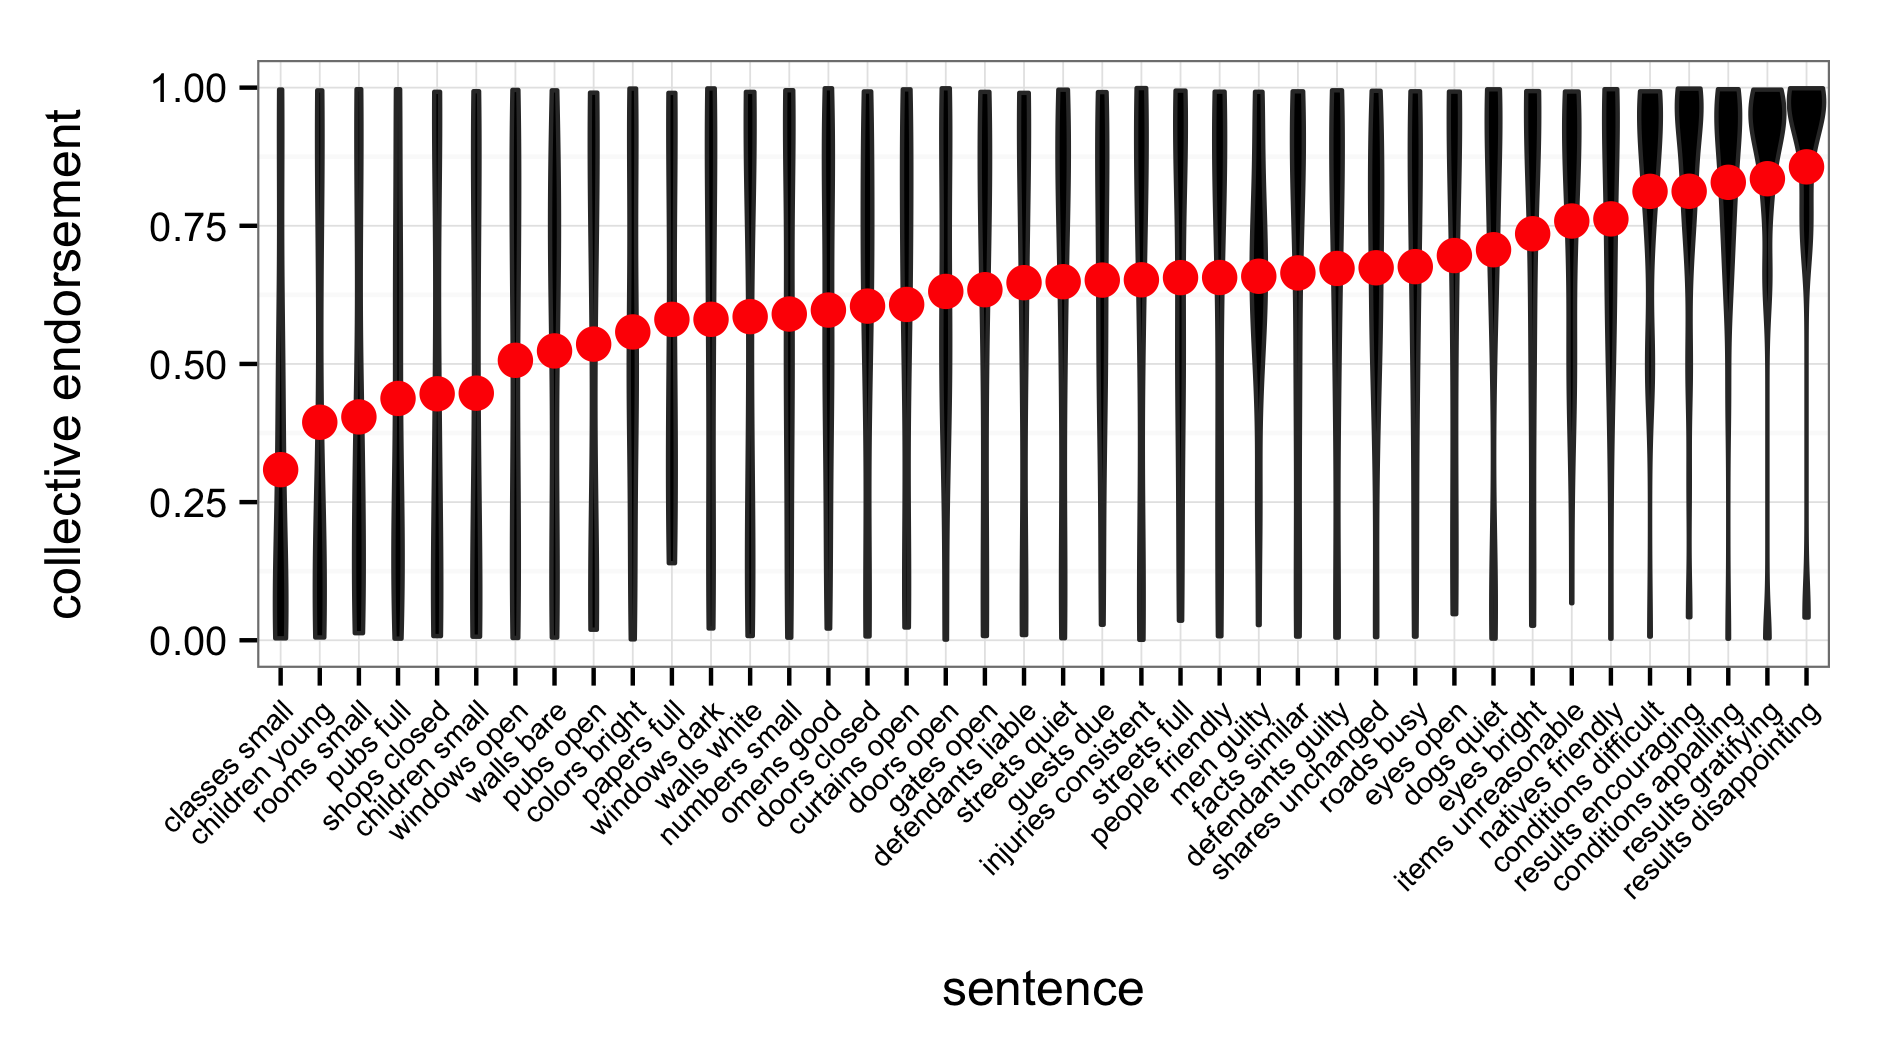
\includegraphics[width=\linewidth]{plots/sentence_plot_violin.eps}

\item \emph{I'm kind of surprised there were only two alternatives considered for the speakers knowledge state: full or sum. It seems to me that the non-regular condition corresponds to a situation that is neither: the speaker has knowledge of the individual boxes, and can kind of vaguely infer what the full set might look like (e.g., by mentally stacking them) but only noisily so.}

We intentionally separated the effects of speaker knowledge and noise in the aggregation of collective properties (by, e.g., mental stacking). Our knowledge manipulation models whether the speaker has access to individual vs. collective properties of the state when choosing to communicate about it. We capture effects of noise explicitly in our noise manipulation, which affects the stability of collective properties. Noise is a property of the communication scenario (i.e., of the world), so it applies to both speakers and listeners equally; we approximate the noise introduced by mental stacking with our noise manipulation.

\item \emph{There needs to be more information about the experimental participants. Nationality? Age? How much were they paid?}

\gcs{got info; how much should we include and where should we put it?}

\een



\subsubsection*{Reviewer 2:}

\emph{General comments}

\ben

\item \emph{The authors should situate their findings against the backdrop of our previous experimental work on \emph{each} and \emph{together}. Haven’t we already established (first theoretically/introspectively, then experimentally across various paradigms) that \emph{each} and \emph{together} disambiguate sentences for adults, and that the interpretation of potentially ambiguous sentences is influenced by pragmatic knowledge?}

All of the previous experimental work that the reviewer mentions investigates post-VP \emph{together} (e.g., \emph{the boxes were big together}), whereas our experiments target post-NP \emph{together} (e.g., \emph{the boxes together were big}). We chose post-NP \emph{together} to avoid the spatiotemporal interpretation of post-VP \emph{together} (cf.~our response to Reviewer 2's point 4 below). While we have followed the reviewer's advice to reference the experiments by Syrett and Musolino, we are careful to highlight the fact that the disambiguating potential of post-NP \emph{together} had not been previously established empirically.

\item \emph{The authors should highlight the role of the speaker's epistemic state.}

\item \emph{The authors set up the contrast between distributive and collective interpretations without mentioning the possibility of cumulative interpretations. This reading should be mentioned.}

\item \emph{The authors repeatedly refer to \emph{together} as though it unambiguously signals a collective interpretation, but this is most definitely not the case!}

The reviewer references previous work that establishes the flexibility of post-VP \emph{together}: as sentence like \emph{the boy and the girl biffed together} allows a spatiotemporal, synchronous distributive interpretation whereby the boy and the girl are close as each of them biffs at the same time. However, we lack evidence of a similar flexibility for post-NP \emph{together}, which is why we used it in our experimental materials and tested its disambiguating potential in Expt.~1. Indeed, the previous experimental work that the reviewer recommended distinguishes the two versions of \emph{together}: 
``post-VP together attaches to the right of the VP and modifies the event, giving rise to multiple interpretations [(i.e., to collective and synchronous distriutive interpretations)], while post-NP together attaches to the left of the VP and requires the predicate in question to apply to the plurality (e.g., John and Mary), giving rise to an obligatorily collective reading'' (Syrett and Muslino, 2016, fn.~1). The consensus in the literature, together with the results of our Expt.~1, suggest that post-NP together does unambiguously signal a collective interpretation, which is why we refer to it as such.

\item \emph{The authors take participants' willingness to accept the sentence \emph{The NOUNS together were ADJECTIVE} as compatible with the speaker's intended meaning as an indication of their willingness to allow a collective interpretation of the target sentence. But this is inherently problematic, because that sentence does not unambiguously signal a collective meaning to the participant! Take the following example: ``The boys together were smiling.'' The true `collective' interpretation of this sentence is that each boy contributed in such a way that collectively the boys created what can be truthfully described as a smiling event, and no one boy has this property, while the group does.}

This point is a continuation of the worry surrounding collective interpretations and \emph{together} expressed in Reviewer 2's points 1 and 4; see above for our arguments that \emph{together} indeed does signal a collective interpretation. The issue of collective smiling is a separate one. To better understand the factors that go into the disambiguation of plural predications, we have chosen to consider in detail a specific class of predicates with (relatively) objective evaluation strategies: gradable adjectives like \emph{heavy} or \emph{big}. 
The measurement inherent to the semantics of these predicates delivers scalar interpretations that are amenable to quantitative study. By examining intuitions about the use of these predicates, together with the predication context that delivers them, we stand to better understand the mechanism of plural predication: when collective interpretations are appropriate, what they communicate, and what mediates the choice between distributive and collective interpretations in the first place. For collective action statements, the evaluation criteria are much less clear, so it is difficult to intuit precisely what these statements entail.\footnote{This is not to say that we know nothing about collective action statements. For example, Margaret Gilbert's Plural Subject Theory makes great gains on this ground in the domain of social philosophy (for a recent overview, see Gilbert, 2013).} However, we disagree with a key aspect of the reviewer's claim, namely that a collective interpretation entails the falsehood of a distributive one. A collective interpretation merely asserts that the plurality holds some property; ``the non-distributive [(i.e., collective)], \emph{together} construal of a sentence doesn't entail the falsehood of the distributive, \emph{each} version'' (Schwarzschild, 1994, p.~212). Just because a distributive interpretation holds true does not preclude a collective interpretation. Whatever it means to collectively smile, it crucially does not mean that there was necessarily no individual smiling. Moreover, in our paraphrase endorsement methodology, participants always rated \emph{both} distributive (i.e., \emph{each}) \emph{and} collective (i.e., \emph{together}) paraphrases; given the choice between ``the boys each smiled'' and ``the boys together smiled,'' it sounds like the reviewer would endorse without hesitation only the distributive paraphrase (an option that was provided to all of our participants).

\item \emph{Participants may have been inserting a silent collectivizing noun (e.g., \emph{box}, \emph{pile}, \emph{stack}) into the \emph{together} sentences.}

While it is impossible to prove the absence of invisible words, we believe this point is related to the potential representational coercion story that we raise in the discussion of Expt.~3: perhaps participants reanalyzed ``the boxes'' as referring to a single individual, that is, to a pile. We have now raised the possibility of silent nouns in the context of our discussion of this point. However, the problem with this story remains the same: the lack of effect for \emph{heavy} (and the other predicates whose dimensions were not targeted in the new Expt.~4); if our predictability manipulation somehow led to reanalysis or the insertion of silent nouns, this should have happened across the board, leading to increased rates of collective interpretations for all predicates. But this is not what we found. Instead, we found increased rates of collective interpretations only when the relevant dimension had been regularized, as predicted by the contextual predictability hypothesis.

\item \emph{A plural definite description like \emph{the boxes} maps onto an atomic join semi-lattice. There is therefore semantically in the representation, a maximal element (just as there is with the singular definite description \emph{the box}). It is entirely possible that participants were predicating of this maximal element, which would make it seem as though they are accessing the collective interpretation, when in fact they are not.}

According to standard theories of the semantics of plurality (e.g., Link, 1983, and subsequent work), a plural definite description like \emph{the boxes} refers to a plural, non-atomic individual (i.e., to a sum of individuals or a non-singleton set, depending on the approach taken); it is nominal predicates (i.e., bare nouns) that map onto atomic join semi-lattices. Plural predication transpires when a plural individual enters into predication; collective predication occurs when we say of a plural individual that it holds the relevant property. Formally, this amounts to asserting that the plural individual is in the denotation of the semantically singular predicate (i.e., a predicate not closed under sum-formation with something like Link's *-operator). Thus, when we ascribe to a plural individual---regardless of whether it is the maximal element of the nominal denotation from which it was drawn---some property directly, we have collective predication.

\item \emph{The authors are aware of the context-dependence of the gradable adjectives that are the target of their investigation (e.g., \emph{big}, \emph{tall}, \emph{heavy}), but they do not make too much of this in the paper. One possibility is that \emph{The boxes (together) are big} could be taken to mean something like, `If you look at the boxes all together, then they form a comparison class such that they surpass some relevant threshold and could be considered to be big.'}

\gcs{it's not clear to me what the point is here}

\item \emph{Don't predicates such as \emph{have brown eyes} have to apply at the atomic level? If so, then aren't there predicates out there for which young language learners must learn that they obligatorily apply to atomic individuals that are members of a plurality? And if this is the case, then couldn't \emph{big} and \emph{tall} be stubbornly distributive at the lexical level?}

We thank the reviewer for bringing this point to our attention. Indeed, there are predicates like \emph{have brown eyes} that appear to necessitate distributive construals. We have added discussion of these so-called ``distributive'' predicates to our introduction, where we lay out the general puzzle. Whereas having brown eyes is a property that necessarily holds of individuals, collective size is not: there is no conceptual barrier to attributing some size directly to a plurality (compare ``the group of men has brown eyes'' with ``the pile of boxes is heavy''). Learning that \emph{have brown eyes} is distributive is tantamount to learning what \emph{have brown eyes} means; not so for stubbornly distributive predicates.

\item \emph{If there are predicates like \emph{gather} that must apply at the level of the group (i.e., they are stubbornly collective) why is it not unreasonable to think that these predicates contrast with another category, whose denotation requires them to apply at the atomic level, and another category, which are flexible in the level to which they apply?}

As with distributive predicates like \emph{have brown eyes} (cf.~our response to Reviewer 2's point 9 above), collective predicates like \emph{gather} name properties that require a collective interpretation by virtue of their meaning. We have added this point to our discussion of the puzzle surrounding stubbornly distributive predicates, whose meanings pose no conceptual barriers to either interpretation.

\item \emph{I am not able to interpret \emph{These boxes are big} collectively. (I am a native speaker of American English.) I can, however, maybe access a collective interpretation of \emph{These boxes are tall}. This paper doesn't allow me to understand why I am encountering an introspective difference between these two predicates, or why we see one in the experimental results.}

\een

\noindent\emph{Other comments}

\begin{enumerate}
	  \setcounter{enumi}{11}

\item \emph{Abstract: The authors say that ``plural predication'' is a source of ambiguity, or should be disambiguated, but what is being disambiguated? Is it the plural predication, or the proposition, or the sentence level? (I revisit this issue of the locus of ambiguity below.)}

\item \emph{Abstract: The phrase ``stubborn distributivity'' should be attributed to Schwarzschild, as it is in the main text.}

We have avoided including references in our abstract. However, we clearly attribute the label ``stubborn distributivity'' to Schwarzschild in the text.

\item \emph{Pg.~3: The transition at the end of the second paragraph is a bit abrupt.}

\item \emph{Pg.~3: Kamp \& Partee (1995) (perhaps among others) should be cited in the second paragraph for properties that depend on the context of predication and comparison classes.}

We have added the suggested citation.
	
\item \emph{Pg.~3: Please revise the description of ``stubborn distributivity'' in the last paragraph. The phenomenon is not about the contrast, as described here, but rather about the observation about the latter class of predicates.}

We have changed the description as suggested.
	
\item \emph{Pg.~4: Champollion (2015)'s proposal about stratified reference seems relevant to this discussion.}

We were unable to reconstruct from this comment the intended connection between Champollion's work on stratified reference and our summary of previous work on stubborn distributivity.

\item \emph{Pg.~4: The term ``complaisantly collective'' is a bit confusing. I think that the authors mean those predicates which allow for both distributive and collective interpretations, but aren't these Link's mixed predicates? These also contrast with collective predicates. (See comments above.)}

We intend ``complaisantly collective'' to describe those predictes, like \emph{heavy}, that admit collective interpretations; we have added this clarification in our revision.

\item \emph{Pg.~4: Using \emph{instantiate} in an intransitive frame seems weird to me (\emph{how regularly they instantiate in the world}, \emph{find objects that instantiate in regular physical arrangements}).}

We have replaced \emph{instantiate} with intransitive \emph{actualize}.
	
\item \emph{Pg.~4: Are the authors claiming in the first paragraph that plural nouns such as \emph{numbers} or \emph{ideas} can admit of collective interpretations with distributive predicates? If so, it would be nice to get some examples.}

\item \emph{Pg.~7, 14, 18, 23: It should be indicated how much participants were compensated.}

\item \emph{Pg.~8: The between-subject inspect/move contrast should be theoretically motivated earlier in section 2.2.}

\item \emph{Pg.~9: The sentence, ``The boxes each were big'' doesn't seem entirely natural to me. More natural would be, ``The boxes were each big.'' I'm assuming the authors wanted the words each and together to appear in the same syntactic position, and that is why they created the sentences in this way, but if that is the case, they should say so, in order to justify their choice of a non-default description that seems slightly unnatural.}

As the reviewer suspected, we chose the post-NP \emph{each} order to minimize the differences between the \emph{each} and \emph{together} paraphrases, and we used post-NP \emph{together} for the reasons discussed above (cf.~our responses to Reviewer 2's points XXX). It isn't clear that either \emph{each} order stands as the default, so we are reluctant to label either as non-default. Indeed, none of our participants expressed concern about the wording of our \emph{each} paraphrase.
	
\item \emph{Pg.~10: Missing the word \emph{accessed} in the first sentence of section 2.4 (\emph{participants chose the collective referent, and therefore accessed the collective interpretation}).}

We have added \emph{accessed} as suggestion.

\item \emph{Pg.~11: Here and elsewhere, ``Appendix'' is mentioned twice in a row.}

We have corrected this error.

\item \emph{Pg.~11: If the difference is not significant, then I don't think the authors are able to mention here and later on (pg. 12) that the results approach significance, or highlight this.}



\item \emph{Pg.~12: If \emph{heavy} is, as the authors say, ``complaisant toward collective interpretations,'' then shouldn't the percentage of `collective' interpretations obtained for this predicate be higher than was observed?}

We ran Expt.~1 in part to establish a baseline of behavior for the three predicates; we make no quantitative predictions on the basis of \emph{heavy}'s complaisant collectivity.

\item \emph{Pg.~13: The authors attribute the difference between the `move' and `inspect' scenarios to the fact that in the latter condition, the speaker does not have as much knowledge about the individual boxes, and so there is a difference in the epistemic state of the speaker. Is this really the key difference? Could it just be that in the `move' scenario, the boxes were moved en masse, and so were clearly treated as a group? The authors should address this possible interpretation of the findings.}

This point is related to Reviewer 2's point 6 about silent nouns. See our response above for reasons why we find it unlikely that participants were treating the boxes as a group \emph{only} in the `move' scenario.

\item \emph{Pg.~13: The ordering presented in the transition between the two paragraphs at the top was a little jolting.} 
	
\item \emph{Pg.~13: Experiment 1 is referred to as a ``reference task'' for what I think is the first time. Presumably this is because the speaker said, ``The boxes are\ldots'' But this was a bit confusing to encounter.}

To avoid this confusion, we now say that Expt.~1 is a reference task when we mention it for the first time in the introduction.

\item \emph{Pg.~14-18: The role of animacy does not appear to have been controlled for in the corpus search in the naturally-occurring or derivative examples. This seems important, and should be addressed. Note that of the examples in (6) on pg. 18, there are more inanimate nouns, and the number varies for each predicate.}

So that we could get a sample of occurrences of plural predication, we intentionally avoided restrictions on our corpus search like animacy of the subject noun. The corpus experiments serve to extend our paraphrase methodology with naturally-occurring examples, and to get a better picture of the empirical terrain of plural predication. We do not intend for the corpus experiments to be robust tests of our hypotheses concerning contextual predictability and speaker knowledge; these hypotheses are tested in Expts.~3 and 4.

\item \emph{Pg.~14-18: The full list of sentences from Experiments 2a, 2b should be provided in an appendix.}

\gcs{Should we do this, or point out that the paper is already too long and the full set of sentences appears in the relevant figures?}

\item \emph{Pg.~14: I'm worried about a circularity in the design of Experiment 2. The authors found highly frequent instances of the sentence template \emph{The NOUNS were ADJ} and created additional examples from these. Participants then chose a paraphrase for these examples. But if the participants are encountering highly frequent examples in the experiment, which presumably have an interpretation paired with them, then aren't they identifying that frequently-intended interpretation in this task?}

Our intention was to investigate the frequently-intended interpretations of plural predications. However, we hesitate to assume that a given sentence has a single interpretation paired with it. In fact, the gradience we observe in our results would suggest against such an assumption.

\item \emph{Pg.~15, 19: The authors filtered out all sentences for which participants reported that the sentences did not `make sense.' I'm not sure why this was done post-hoc, instead of via a pre-experiment norming task. The 67\% `made sense' reported in Experiment 2b seems quite low to me. I would like to request that the authors to include a note about this.}

The 67\% `made sense' rate was for the novel sentences that participants encountered in Expt.~2a. These novel sentences served as fillers so that participants were not only encountering highly-frequent sentences. However, our analyses look only at the highly-frequent sentences, and participants indicated that these made sense 95\% (Expt.~2a) and 98\% (Expt.~2b) of the time. To avoid confusion, we have moved our mentions of the `made sense' rates for the filler sentences to footnotes.

\item \emph{Pg.~16, figure 4: What should be made of the near-50 to 60\% ratings/endorsement of the vast majority of the sentences? This seems troublesome to me.}

We are careful not to conclude anything on the basis of the specific mean collective endorsement rating for any given predicate. What we do conclude is that there are no clear groupings of predicates that would suggest the categorical distinction implied by stubborn distributivity.

\item \emph{Pg.~16, figure 4: I am still completely confused as to how certain sentences as indicated on the x axis, such as those created by the combination of eyes-open, natives-friendly, walls-white, etc.) are really given a collective reading. What exactly does this mean? In each of these instances, don’t the atomic individuals still have to have the property – if not all of them, then some near-maximal amount?}

We believe the confusion arises here because of certain atypical assumptions the reviewer is making about collective interpretations. Please see our response to Reviewer 2's point 5 above.

\item \emph{Pg.~18: I am concerned that the \emph{lids} noun in (6) is really eyelids (and not lids of containers), and therefore the `lids' are not literally ‘heavy’. These examples came from the Google Books corpus, so I think it is entirely possible that this is the case.}

It certainly is possible that our corpus search identified tokens of `lids' wherein the noun refers to eyelids. When we excluded abstract interpretations, we were looking at our specific sentence frame (e.g., ``the rains were heavy'' or ``the casualties were heavy''). There is a perfectly reasonable literal, non-abstract interpretation for ``the lids are heavy.'' 

\item \emph{Pg.~18: I am also curious about the \emph{trees-heavy} pairing indicated here. What are these sentences in which trees are described as being `heavy'? Are they instead sentences describing the trees as being `heavy with fruit'? If so, again, this seems like a different sort of sentence and non-literal use of heavy.}

As in our response to the previous point, at issue is the readily-accessible interpretation for ``the trees were heavy'' whereby the speaker comments on the weight of trees. Here is a post-test quote from one of our participants that summarizes the issue nicely: ``I'm sometimes unsure what is being asked when the question is `does the sentence make sense?'  Sentences such as `The houses are heavy,' are uncommonly needed (!), but if a house was being moved off its foundation, it might be used.  Same with the trees being heavy -- maybe they're on a logging truck.  But in day to day speech, no, you wouldn't hear these sentences.''

\item \emph{Pg.~18: A similar concern might be raise about \emph{big-boys}, which has two interpretations.}



\item \emph{Pg.~19-20: I would have expected the \% `collective' associated with \emph{heavy} to be higher, and would have liked for the authors to say a little more about the relatively low \% observed.}

We ran these experiments so that we could calibrate our (and the reader's) expectations. A semanticist who identifies `heavy' as one of the few gradable predicates that allows a collective interpretation would likely have an inflated sense of the predicate's collective interpretation rate.
	
\item \emph{Pg.~19-20: The \% `collective' for \emph{big} and \emph{tall} sure looks like an indication of ``stubborn distributivity''+noise to me! If the authors think that the results should not be interpreted in this way, I think they should address this possible interpretation head on.}

We address this possible interpretation head-on in the \emph{Results} section of Expt.~2b: ``We might take the split in behavior between \emph{heavy} on the one hand and \emph{big} and \emph{tall} on the other as evidence for a categorical divide between complaisantly collective and stubbornly distributive predicates. However, comparing the predicates at the level of individual subject nouns suggests otherwise\ldots''

\item \emph{Pg.~25: If I understand Figure 8 correctly, participants were given the paraphrase sentences one on top of the other, and asked to slide the scale for each sentence. Did the scale start at 0 or 50 for each? More importantly, why present the sliding scales next to each other and not across items? I worry that this setup precludes them from allowing both to be rated highly, and that they should complement each other (which is what it looks like in Figure 9).}

The leftmost point on the scale (corresponding to `definitely not') was coded as 0; the rightmost point (corresponding to `definitely') was coded as 1. We presented the sliding scales next to each other, rather than across items, to highlight the potential ambiguity of the test sentences.

\item \emph{Pg.~29: The authors should explain what they mean by saying that the collective and distributive senses as `vague expressions.'}

\item \emph{Pg.~31: The authors' point that the speaker ``chooses an utterance u that would most effectively communicate some state s to a literal listener'' seems to me to indicate that the speaker will take
into account morphosyntactic and structural information when doing so, which is a point that Syrett \& Musolino (2015) have made when discussing the disambiguation of sentences with possible collective and distributive senses. The authors do not really discuss such structural/surface level cues, but should acknowledge them, because they figure into the form of the utterance chosen by the speaker.}

\item \emph{Pg.~31: The authors say that the speaker's belief distribution about the state of the world depends on ``some observations o of the true world.'' Is this way of phrasing things meant to privilege perceptual over conceptual information?}

\item \emph{Pg.~32: Why is the variability of the context considered a semantic factor?} 

\item \emph{Pg.~32: Please explain the degrees in section 5.2.}

\item \emph{Pg.~34: The wording ``an old observation about collective interpretations for gradable predicates with plural subjects'' makes me wonder at what level the authors see the ambiguity being encoded (the VP level or the sentence level), so it might be helpful to add a note somewhere about this, since there have been different approaches to the semantic treatment of the collective/distributive ambiguity over the years. (The comment in the top paragraph on pg.~38 about the locus of ambiguity is also related to this point.)}



\item \emph{Pg.~36: The authors suggest that, ``stubbornly distributive predicates name collective properties that are difficult to accurately communicate.'' By this point in the paper, I am so far from convinced that the participants are really accessing a true collective reading, that on this page, I am not on board with the conclusions, and am certainly not in agreement with this claim, even though I do agree with the authors that the context is able to bring out readings that are otherwise suppressed, and I think the experiments presented in the paper do a nice job of showing that this is the case. Whether or not these non-strictly-distributive readings can really be taken to be collective readings is another matter.}



\item \emph{Pg.~38: I would think that if the noun phrase is construed as an aggregate (i.e., a single collection) instead of a group, then the predicate is no longer applying to the group, but rather to the collectivizer, in which case we return to the possibility that participants may have inserted a silent collectivizing noun into their interpretation of the sentences.}

Please see our responses to Reviewer 2's points 6 and 28 above.

\end{enumerate}


\subsubsection*{Reviewer 3:}

\ben

\item \emph{p.~3: Piano example in first paragraph: I'm not convinced this is a good example. In the first sentence, ``piano'' is singular so there's one piano and no ambiguity about it; it isn't obvious that there is a problem to be solved from this example. The example with ``the boxes are heavy'' vs.~``the boxes are big'' is much more compelling.}
	
We have removed this example.

\item \emph{p.~4:~``Second, it leaves unexplained why some predicates would contain pluralities and others not—is there a deeper explanation in terms of the properties named?'' An obvious null hypothesis here is that stubborn distributivity is randomly distributed across classes of adjectives; in that case there is nothing to be explained. You can motivate against this hypothesis here by noting cross-linguistic similarities in which classes of adjectives are stubbornly distributed.}

We chose to avoid discussing this straw-man hypothesis in order to keep focus on our actual hypothesis and in an attempt to keep our already-too-long paper short.

\item \emph{p. 5 top: The logic in this paragraph is hard to follow. Initially I didn't understand why ``the collective use of tall would be more likely to mislead a listener than that of heavy'' -- if I say ``the boxes are tall'' and mean it distributively, surely that conveys that the boxes are in an arrangement such that they are tall? And if their arrangement *is* already in common ground, then what utility is there in saying they are tall?
Is the logic that there are many different ways in which the boxes could be tall, so ``tall'' is not very informative? 
In RSA terms, it was helpful for me to think of this first p. at the level of L1, whereas the exposition here seems to be going back and forth between S1 and L1. I think I got confused because of things like ``collective interpretations will be avoided by speakers'' -- it's confusing to talk about speakers choosing an interpretation.}

We have attempted to clarify our point by highlighting the possibility that a speaker and listener could encounter the relevant plurality in differing arrangements. As for speaker's choosing interpretations, our model of utterance disambiguation has the utterance-generation process (i.e., $S_1$) proceed with a fixed interpretation; $L_1$, the real-world listener, reasons about this process in interpreting an underspecified (i.e., ambiguous) utterance: what would that speaker have been most likely to have intended?

\item \emph{How was heaviness represented in the questions?}

Heaviness was represented visually.

\item \emph{p.~10 bottom: ``Appendix Appendix A''}

We have corrected this error.

\item \emph{p.~11: Why the small effect of scenario on interpretation of ``heavy''? Maybe the participants weren't paying much attention to the scenario?}

We speculate on the lack of a significant effect of the scenario manipulation later in our paper (cf.~our response to Reviewer 3's point 12 below). Given that we had the same manipulation in our Expt.~3 and found a significant effect there, we doubt that participants were simply ignoring it.

\item \emph{p.~15: 11Appendix Appendix B''}

We have corrected this error.

\item \emph{p.~16: The black-on-black error bars are hard to see.}

We have lightened the bars to improve visibility.

\item \emph{For experiment 2, I wonder if some of the nouns are really plural (\emph{conditions}, \emph{results}).}

This is a reasonable concern about our corpus-based experimental items, which we selected solely on the basis of frequency of occurrence. We ran the follow-up in Expt.~2a with a more targeted set of items in part to allay this concern. There, subject nouns denoted real-world (as opposed to abstract or psychological) entities.

\item \emph{For experiment 2, some of the collective interpretations imply a distributive one (\emph{the dogs were quiet}). This is an interesting factor, which is graded among nouns, which is not discussed so far.}

We agree that this factor is interesting, but we have chosen to leave its exploration to future work.

\item \emph{p.~20: ``Appendix Appendix B''}

We have corrected this error.

\item \emph{p.~23: ``It is possible that this effect was real, but small because of a bias for the distributive referent (leading to a floor effect)'' -- are you proposing that this bias is part of the prior distribution on meanings for this word? Or do you mean a general across-the-board bias toward distributive referents given the experimental setup?}

We meant the latter interpretation.

\item \emph{p.~26: ``Appendix Appendix C''}

We have corrected this error.

\item \emph{In experiment 3's irregular conditions, maybe the participants are thinking: Cubert wouldn't say the boxes were collectively tall unless they were collectively VERY tall; so here he must have been referring to the individual boxes. Admittedly, I'm not sure how this would apply to ``big''. This alternative story suggests that you should control for the actual height of the boxes when predicting responses. Maybe the difference between ``regular'' and ``irregular'' conditions just reflects the difference in total average height in the ``tall'' case.}

The results of our new experiment (\emph{Expt.~4: Generalizing our findings}) explore and support this intuition: the probability that a specific interpretation would truthfully describe a state of affairs enters into the pragmatic calculus of utterance disambiguation. As suspected, interpretations that are more likely to be true (e.g., a collective interpretation for \emph{narrow} with a tall, thin stack of boxes) are more likely. We expand on this finding in our discussion of Expt.~4's results.

\item \emph{p.~32: isn't alpha=7 fairly high for these models? In general, it would be nice to see some figures showing how ``the qualitative patterns reported below are robust to changes in these parameters and assumptions.''}

There isn't yet a sense of what counts as high or low for the optimality parameter $\alpha$ in RSA models. Rather than discussing alternative parameter settings at length with accompanying plots, we chose to link to the full model, where the interested reader can manipulate the parameters and assumptions on their own.

\een


\newpage

\noindent Thank you again for the thorough and thoughtful comments on our work. We hope that you will like the new version of the paper. Please let us know if you require additional information. We look forward to hearing from you!\\[25pt]


\noindent Yours sincerely,\\[10pt]

\noindent Gregory Scontras and Noah D.~Goodman



\end{document}














